% QEX Preprint — v0.1.0
% "Plumb Correction of a Leaning Antenna Mast by Rotated-Bearing Geometry"
% KD7VDG — Portland Amateur Radio Club (W7LT)
% Submitted for consideration to QEX, ARRL's Forum for Communications Experimenters
%
% NOTE TO REVIEWERS: This is a preprint. Figures, final citation cross-checks,
% and confirmation measurements (pipe OD, bracket standoff) are pending Trip 2.
%
\documentclass[11pt,twocolumn]{article}

\usepackage[margin=1in,top=1.1in,columnsep=0.25in]{geometry}
\usepackage{amsmath,amssymb}
\usepackage{tikz}
\usetikzlibrary{calc,arrows.meta,decorations.markings}
\usepackage{xcolor}
\usepackage{booktabs}
\usepackage{enumitem}
\usepackage{fancyhdr}
\usepackage{hyperref}
\usepackage{graphicx}

\hypersetup{colorlinks=true, linkcolor=blue!60!black, urlcolor=blue!60!black,
  citecolor=blue!60!black}

\definecolor{polecolor}{RGB}{110,80,48}
\definecolor{pipecolor}{RGB}{50,140,200}
\definecolor{okgreen}{RGB}{20,160,80}
\definecolor{goldhl}{RGB}{200,150,20}
\definecolor{warnred}{RGB}{200,60,60}

\pagestyle{fancy}
\fancyhf{}
\lhead{\small\textit{QEX Preprint} --- \textsc{kd7vdg}}
\rhead{\small\textit{Antenna Mast Plumb Correction} --- March 2026}
\cfoot{\small\thepage}
\renewcommand{\headrulewidth}{0.4pt}

% QEX-style: no section numbering, flush-left headings
\setcounter{secnumdepth}{0}

% -----------------------------------------------------------------------
\begin{document}
% -----------------------------------------------------------------------

\twocolumn[{%
\begin{center}
  {\LARGE\bfseries Plumb Correction of a Leaning Antenna Mast\\[4pt]
  by Rotated-Bearing Geometry}\\[10pt]
  {\large KD7VDG --- Portland Amateur Radio Club (W7LT)}\\[4pt]
  {\normalsize Portland, Oregon $\cdot$ March 2026}\\[6pt]
  {\small\textit{Preprint v0.1.0 --- submitted for consideration to QEX}}
\end{center}

\medskip
\hrule
\smallskip

\begin{quote}\small
\textbf{Abstract.}
A Motorola Quantar repeater with a sector antenna requires a plumb mounting
mast. The W7LT repeater site at Mt.\ Scott uses a wooden telephone pole that
has developed a lean of $9.46^\circ$ from vertical. The conventional remedies
(shims, standoff blocks, guy wires) were ruled out by site constraints. This
article presents a geometrically elegant alternative: rotating the lower
bracket bearing around the pole's circumference by a calculated angle so that
the chord connecting the two bracket attachment points is vertical. The
solution requires no new hardware beyond replacement all-thread and backing
plates. The geometry is derived from first principles using the chord-of-a-circle
relationship. A field procedure using gravity and ballast eliminates measurement
error in the lean direction. The same geometry is extended to cover wind loading,
cantilever ratio, and clearance margin. A follow-on system for continuous
structural health monitoring using MEMS accelerometers and Elixir/Phoenix is
briefly described.
\end{quote}

\smallskip
\hrule
\bigskip
}]

% -----------------------------------------------------------------------
\section{Background}
% -----------------------------------------------------------------------

Sector antennas have a pattern that depends critically on vertical orientation.
A few degrees of tilt shifts the horizontal beam downward on one side, dumping
signal into a hillside, and upward on the other, overshooting the coverage area.
For a hilltop repeater serving a metropolitan area, even a $3^\circ$ error in
vertical alignment causes measurable coverage degradation.

The W7LT club's site on Mt.\ Scott in southeast Portland, Oregon, supports a
Motorola Quantar repeater on 147.18~MHz. The antenna mast is a 3-inch OD
galvanized steel pipe fastened to a wooden telephone pole with two U-bolt
saddle clamp brackets. Over time, the wooden pole has developed a lean. A field
survey on 28 February 2026 by KJ6VU, WA7NE, and the author measured the lean
at approximately $9.5^\circ$ from vertical---too much to ignore, and directly
in conflict with the sector antenna installation that is planned.

The obvious fixes have problems. Shimming the brackets requires knowing the exact
lean direction and magnitude at the bracket heights, fabricating asymmetric
standoffs, and re-drilling. Guy wires are not permitted on this site, which is
on city water department property adjacent to a commercial tower farm. Replacing
the pole is a major infrastructure project out of scope for a club installation.

What I was looking for was a solution that used the hardware we already had,
required minimal new material, and could be self-verifying in the field without
precision instruments.

% -----------------------------------------------------------------------
\section{Field Survey}
% -----------------------------------------------------------------------

The survey used a simple plumb drop: a weight on a string was suspended from
each bracket height and the string's contact point with the ground was marked
with a stone. Horizontal distances between the stone pairs were measured with
a tape in the north--south and east--west directions and confirmed by direct
diagonal measurement.

\begin{table}[h]
\centering\small
\begin{tabular}{@{}lr@{\enspace}l@{}}
\toprule
Parameter & Value & Notes \\
\midrule
Wooden pole diameter & $7.5''$ & \\
Pipe outside diameter & $3.0''$ & to confirm, Trip 2 \\
Bracket standoff gap & $4.5''$ & fist-width at bracket \\
Bracket spacing & $36''$ & current configuration \\
Plumb drop N--S & $6.0''$ & \\
Plumb drop E--W & $2.0''$ & see text \\
Plumb drop diagonal & $6.0''$ & direct measurement \\
\bottomrule
\end{tabular}
\caption{Field measurements, 28 Feb 2026.}
\label{tab:field}
\end{table}

The N--S and E--W components, if exact, would give a diagonal of
$\sqrt{6^2 + 2^2} \approx 6.32''$, not $6.0''$. A diagonal of $6.0''$ is
consistent with a nearly pure north--south lean and a small (possibly
measurement-noise) east--west component. The direct diagonal measurement is
the most reliable number---fewest intermediate steps---so I use $\delta = 6.0''$
as the total lean displacement. The ballast method described in the procedure
section corrects for the lean in all directions simultaneously regardless of
how the components resolve.

\textbf{Orbit radius.} The pipe center is not at the pole surface; it stands
off from the pole at a distance set by the bracket hardware. From the pole axis
to the pipe center:
%
\begin{equation}
  R = r_\text{pole} + g + r_\text{pipe} = 3.75 + 4.5 + 1.5 = 9.75''
  \label{eq:R}
\end{equation}
%
I call this the \emph{orbit radius}. The pipe center sits on a circle of this
radius centered on the pole axis. If the bracket hardware were rotated around
the pole, the pipe center would trace that circle.

\textbf{Lean angle.} From the plumb drop over the $36''$ bracket span:
%
\begin{equation}
  \alpha = \arctan\!\bigl(\tfrac{6}{36}\bigr) = 9.46^\circ
  \label{eq:alpha}
\end{equation}
%
This is a property of the pole. At any bracket spacing $L'$, the lean
displacement is $\delta' = L' \tan \alpha = L' / 6$.

% -----------------------------------------------------------------------
\section{The Rotated-Bearing Solution}
% -----------------------------------------------------------------------

\subsection{Concept}

Both brackets currently clamp the pipe at the same compass bearing around the
pole: the all-thread rods at each bracket pass through the pole on parallel
horizontal axes. Because the pipe is held at the same relative position to the
(leaning) pole at both bracket heights, the pipe leans with the pole.

The correction is to rotate the lower bracket's all-thread to a \emph{different}
compass bearing. This shifts the pipe's lower attachment point horizontally.
With the correct rotation angle, the line connecting the upper and lower
attachment points is vertical---and the pipe hangs plumb.

Figure~\ref{fig:topdown} shows this as a top-down view. The upper bracket
places the pipe at a fixed point on the orbit circle. The lower bracket is
rotated by $\theta$ around that circle. The two points are connected by a
straight line (the pipe), which is a chord of the orbit circle.

\subsection{Derivation}

For a circle of radius $R$, the chord length $c$ subtended by a central angle
$\theta$ is the standard half-angle result:
%
\begin{equation}
  c = 2R\sin\frac{\theta}{2}
  \label{eq:chord}
\end{equation}
%
For the pipe to be vertical, this chord must equal the horizontal lean
displacement $\delta'$ between the two bracket heights:
%
\begin{equation}
  \theta = 2\arcsin\frac{\delta'}{2R}
  \label{eq:theta}
\end{equation}
%
This has a solution as long as the lean does not exceed the orbit diameter:
$\delta' \leq 2R$.

\subsection{Midspan Clearance}

The pipe runs as a straight line (chord) between the two bracket attachment
points. Because a chord passes inside the circle it subtends, the pipe is
closest to the pole at midspan. Setting up the parametric midpoint geometry
and applying the half-angle identity:
%
\begin{equation}
  d_\text{min} = R\cos\frac{\theta}{2}
  \label{eq:clearance}
\end{equation}
%
The pipe clears the pole when $d_\text{min} > r_\text{pole} + r_\text{pipe}
= 5.25''$.

% TOP-DOWN FIGURE
\begin{figure}[h]
\centering
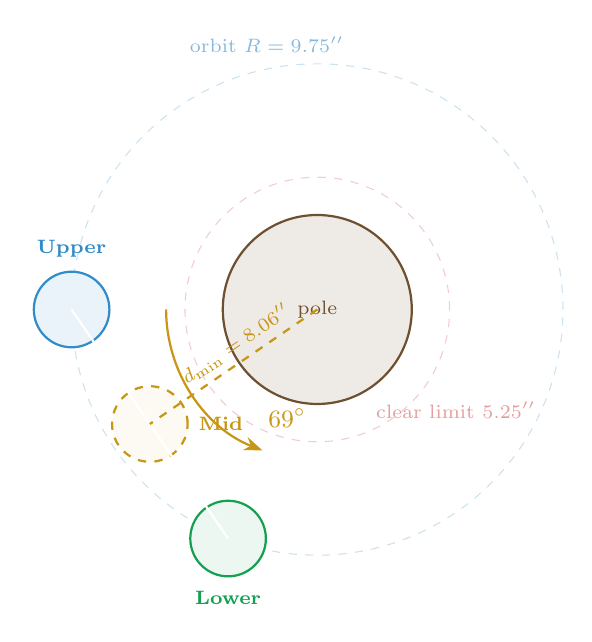
\begin{tikzpicture}[scale=0.32]
  % Pole
  \draw[thick, polecolor, fill=polecolor!12] (0,0) circle (3.75);
  \node[polecolor, font=\scriptsize] at (0,0) {pole};
  % Orbit circle
  \draw[dashed, pipecolor!25] (0,0) circle (9.75);
  % Clearance limit
  \draw[dashed, warnred!25] (0,0) circle (5.25);
  % Upper bracket (angle 180)
  \draw[thick, pipecolor, fill=pipecolor!10] (-9.75, 0) circle (1.5);
  \node[pipecolor, font=\scriptsize, above] at (-9.75, 1.7)
    {\textbf{Upper}};
  % Lower bracket (rotated 68.7 deg → angle 248.7)
  \draw[thick, okgreen, fill=okgreen!8] (-3.54, -9.09) circle (1.5);
  \node[okgreen, font=\scriptsize, below] at (-3.54, -10.8)
    {\textbf{Lower}};
  % Midspan
  \draw[thick, goldhl, dashed, fill=goldhl!5] (-6.645, -4.545) circle (1.5);
  \node[goldhl, font=\scriptsize, right] at (-5.1, -4.545)
    {\textbf{Mid}};
  % Chord (pipe path)
  \draw[white, thick] (-9.75, 0) -- (-3.54, -9.09);
  % Clearance at midspan
  \draw[goldhl, thick, dashed] (0,0) -- (-6.645, -4.545);
  \node[goldhl, font=\scriptsize, rotate=34, above] at (-2.8,-2.0)
    {$d_{\min}=8.06''$};
  % Rotation arc
  \draw[-{Stealth}, goldhl, thick] (-6,0) arc (180:248.7:6);
  \node[goldhl, font=\small] at (-1.2,-4.3) {$69^\circ$};
  % Orbit label
  \node[pipecolor!60, font=\scriptsize] at (-2, 10.5)
    {orbit $R=9.75''$};
  % Clearance label
  \node[warnred!50, font=\scriptsize] at (5.5, -4)
    {clear limit $5.25''$};
\end{tikzpicture}
\caption{Top-down view of the pole cross-section. The upper bracket (blue)
and lower bracket (green) are both on the orbit circle, separated by $69^\circ$.
The chord (white, the pipe) passes through the midspan position (gold dashed).
The minimum pole-to-pipe-center distance is $8.06''$, well above the $5.25''$
clearance limit.}
\label{fig:topdown}
\end{figure}

% -----------------------------------------------------------------------
\section{Recommended Configuration}
% -----------------------------------------------------------------------

\subsection{Cantilever Ratio}

The pipe extends above the upper bracket as an unguyed cantilever. Wind on the
cantilever creates a bending moment resisted by the bracket pair. Standard
structural practice and antenna installation references \cite{ARRLAntenna,TIA222}
characterize this as the cantilever ratio $k = h/s$, where $h$ is the
cantilever length above the upper bracket and $s$ is the bracket span.

For a uniform distributed wind load $w$ on the cantilever, summing moments
about the upper bracket gives the lower bracket reaction force:
%
\begin{equation}
  F_\text{lower} = \frac{wh^2}{2s}
  \label{eq:Flower}
\end{equation}
%
and summing horizontal forces gives the upper bracket force:
%
\begin{equation}
  F_\text{upper} = wh\!\left(1 + \frac{h}{2s}\right) = wh\!\left(1 + \frac{k}{2}\right)
  \label{eq:Fupper}
\end{equation}
%
At an exposed hilltop site like Mt.\ Scott---elevation $\sim 1{,}000$~ft,
subject to Columbia Gorge wind events---the conservative ratio $k = 1.0$
is recommended for an unguyed mast. This keeps $F_\text{upper} \leq 1.5\,wh$.

\subsection{Geometry at the Recommended Span}

With the 12-foot pipe, a 12-inch tail below the lower bracket, and $k = 1.0$:
%
\begin{equation}
  s = h = \frac{144'' - 12''}{2} = 66''
\end{equation}
%
The lean displacement at the new 66-inch span:
%
\begin{equation}
  \delta' = 66 \times \tan(9.46^\circ) = 11.0''
\end{equation}
%
The required rotation angle:
%
\begin{equation}
  \theta = 2\arcsin\frac{11.0}{2 \times 9.75} = 2\arcsin(0.564) = 68.7^\circ
\end{equation}
%
Midspan clearance:
%
\begin{equation}
  d_\text{min} = 9.75\cos(34.3^\circ) = 8.06''
\end{equation}
%
Margin over the $5.25''$ clearance limit: $\mathbf{2.81''}$.

\subsection{Wind Load Check}

Wind force per unit length on a 3-inch cylinder at 60~mph design wind
\cite{ASCE722}:
%
\begin{equation}
  w = \tfrac{1}{2}(0.00238)(88)^2(1.2)(0.25) = 2.76~\text{lb/ft}
\end{equation}
%
where $0.00238$~slug/ft$^3$ is the standard sea-level ISA air density
\cite{ISA1975}. At Mt.~Scott's elevation of $\sim\!1{,}000$~ft, the actual
density is approximately $0.00231$~slug/ft$^3$ ($-3\%$); the sea-level value
is used as a conservative upper bound.
%
At $s = h = 5.5$~ft:
\begin{align*}
  F &= 2.76 \times 5.5 = 15.2~\text{lb (total wind on cantilever)} \\
  F_\text{upper} &= 15.2 \times 1.5 = 22.8~\text{lb}
\end{align*}
%
A single $\tfrac{1}{2}''$-13 Grade~2 all-thread rod has a proof load of
approximately 1,900~lb \cite{SAE429}. At 22.8~lb the safety factor exceeds
$80\times$. The limiting structural element is the bearing strength of the
wooden pole at the backing plate contact---which is why $3'' \times 3''$ steel
backing plates are specified, not the all-thread.

\subsection{Sensitivity to Measurement Uncertainty}

The standoff gap and pipe diameter will be confirmed on the next site visit.
Table~\ref{tab:sensitivity} shows the solution is robust across all plausible
combinations: even the worst case ($g = 3.0''$, $D_m = 2.5''$) clears with
over an inch of margin.

\begin{table}[h]
\centering\small
\begin{tabular}{@{}rrrrl@{}}
\toprule
$g$ & $D_m$ & $R$ & $\theta$ & Margin \\
(in) & (in) & (in) & (deg) & (in) \\
\midrule
3.0 & 2.5 & 8.00 & 86.9 & 1.13 \\
3.0 & 3.0 & 8.25 & 83.6 & 1.42 \\
4.0 & 2.5 & 9.00 & 75.4 & 2.23 \\
\rowcolor{gray!10}
4.5 & 3.0 & 9.75 & 68.7 & 2.81 \\
5.0 & 3.0 & 10.25 & 64.9 & 3.36 \\
\bottomrule
\end{tabular}
\caption{Sensitivity to bracket gap and pipe diameter at the
66-inch span. Highlighted row: best estimate. All combinations pass.}
\label{tab:sensitivity}
\end{table}

% -----------------------------------------------------------------------
\section{Field Procedure}
% -----------------------------------------------------------------------

The most important insight in the procedure is that you do not need to
calculate the exact direction of the new hole in the field. You can let
gravity do it.

\begin{enumerate}[leftmargin=*, itemsep=4pt, label=\arabic{*}.]
\item \textbf{Confirm measurements.} Tape the pipe OD and bracket standoff at
  both bracket heights. Consult Table~\ref{tab:sensitivity} for the clearance
  margin with the measured values.

\item \textbf{Mark pipe positions.} If the pipe is to be raised, mark the
  desired final bracket positions on the pipe before loosening anything.

\item \textbf{Hang ballast.} Attach 25--40~lb (sandbag or concrete mix bag)
  to the bottom of the pipe with a ratchet strap while all brackets are tight.

\item \textbf{Loosen the lower bracket.} Leave it snug enough to prevent
  uncontrolled swinging but free to slide against the pole.

\item \textbf{Loosen the upper bracket.} The pipe now hangs from the upper
  bracket with the ballast pulling it toward plumb.

\item \textbf{Mark the new bearing.} With the pipe hanging plumb, note where
  the lower bracket hardware contacts the pole. This is the correct bearing---
  gravity has resolved the two-axis lean into a single correct point with no
  trigonometry required. Mark the pole surface with a lumber crayon.
  Have a ground crew member confirm plumb from two perpendicular sightlines.

\item \textbf{Drill the new hole.} Use a $\tfrac{9}{16}'' \times 12''$ ship
  auger bit to drill through the pole at the marked bearing, $3''$--$4''$
  below the existing lower hole (which is left in place).

\item \textbf{Install new all-thread.} Pass $\tfrac{1}{2}''$-13 all-thread
  through the new hole with $3'' \times 3'' \times \tfrac{1}{4}''$ steel
  backing plates on both sides. Finger-tight only at this stage.

\item \textbf{Mount lower bracket, re-snug upper bracket.} The upper bracket
  stays at its current pole bearing; no changes are needed there.

\item \textbf{Verify plumb and torque.} Torpedo level from two perpendicular
  sides, confirmed by ground crew sighting. When plumb is confirmed, final-torque
  all hardware.

\item \textbf{Remove ballast.} Mount antenna. Dress coax.
\end{enumerate}

\subsection{Why the Ballast Method Works}

The lean has components in both the N--S and E--W axes. Computing the combined
lean bearing analytically from field tape measurements in grass, with a plumb
bob in wind, introduces compounded uncertainty. The ballast method sidesteps
this entirely: a weight on the pipe defines plumb by physical law. The pipe's
contact point at the lower bracket height shows the correct hole bearing in
both axes simultaneously. The result is self-verifying: if the pipe looks plumb
from two perpendicular sightlines, it is plumb.

% -----------------------------------------------------------------------
\section{Discussion}
% -----------------------------------------------------------------------

\subsection{Why This Works: The Role of Orbit Radius}

The large standoff gap ($g = 4.5''$) is what makes the rotated-bearing approach
viable. It gives a large orbit radius ($R = 9.75''$), which means a moderate
rotation angle produces a large horizontal displacement of the pipe center. The
chord at $\theta = 68.7^\circ$ produces the required 11-inch correction with
plenty of midspan clearance.

If the pipe were clamped directly against the pole surface ($g \approx 0$,
$R \approx 5.25''$), the same calculation at the 66-inch span would require
$\theta \approx 95^\circ$, producing a midspan clearance below the pipe--pole
surface limit. The solution fails. The standoff hardware that initially looks
like mechanical excess is precisely what enables the elegant geometric
correction.

\subsection{Scale Invariance of the Clearance Problem}

An intuitive but incorrect approach is to move the lower bracket further down
the pole to increase the span and thereby reduce the correction needed. This
does not work. The lean displacement grows linearly with span (Eq.~\ref{eq:alpha}),
so increasing the span increases $\delta'$ proportionally. Substituting into
the clearance formula:
%
\begin{equation}
  d_\text{min} = \sqrt{R^2 - \frac{\delta'^2}{4}}
  = \sqrt{R^2 - \frac{L'^2\tan^2\alpha}{4}}
\end{equation}
%
Any increase in span $L'$ decreases $d_\text{min}$. Increasing the span always
worsens the clearance.

\subsection{Adjustability for Future Lean Changes}

Wooden poles continue to lean. The rotated-bearing approach is inherently
adjustable: if the lean changes, a new hole at a different bearing is drilled
and the bracket relocated. Old holes are structurally neutral provided they are
spaced at least $2.5''$ center-to-center \cite{NDS2024}. The pole is not
consumed by corrections.

% -----------------------------------------------------------------------
\section{Continuous Structural Health Monitoring}
% -----------------------------------------------------------------------

The field survey answered the question ``how much has the pole leaned?'' It
cannot answer: ``is the lean increasing?'', ``at what rate?'', or ``is a wind
event in progress right now?'' A follow-on project will deploy a continuous
structural health monitoring (SHM) system at the site. The same first-principles
rigor that informs the mechanical correction---asking what you actually need
to measure and why---informs the sensor selection.

The architecture is two-tier: an ESP32-S3 sensor node on the pole (solar +
LiPo powered, MEMS IMU, MQTT over WiFi) feeds a Raspberry Pi hub in the shack
running a Phoenix/Elixir application, PostgreSQL with TimescaleDB for the time
series, and Phoenix LiveView for a kiosk display. Threshold-based alerts
dispatch email, SMS, or APRS telemetry.

A central research question in that project is \emph{how much sensor do you
actually need?} Four tiers of MEMS accelerometers will be deployed
simultaneously on a rigid plate: the MPU-6050 (\$12, $\pm 0.5^\circ$) as the
cost floor; the ICM-20948 (\$17) and BNO055 (\$30) as intermediate grades;
and the Analog Devices ADXL355 ($25\,\mu\text{g}/\sqrt{\text{Hz}}$, sub-$0.01^\circ$
with averaging) as the reference standard. Noise characterization by Allan
variance, thermal sensitivity, and calibration transfer across tiers will form
the basis of a comparative metrology study---the same measurement science
philosophy applied to lithography stage positioning, six orders of magnitude
less stringent in specification.

That work will be the subject of a follow-on article.

% -----------------------------------------------------------------------
\section{Conclusion}
% -----------------------------------------------------------------------

A wooden pole leaning at $9.46^\circ$ can be corrected for antenna mounting
by rotating the lower bracket bearing $68.7^\circ$ around the pole
circumference and increasing the bracket span to $66''$. The solution requires
no shims, standoff blocks, or guy wires. The existing bracket hardware provides
the standoff geometry that makes pure rotation viable. A ballast-and-gravity
field procedure determines the correct hole bearing without computation, and is
self-verifying. Wind loading at $k = 1.0$ produces bracket forces under 23~lb
against an all-thread proof load of 1,900~lb. The pipe clears the pole at
midspan with $2.81''$ to spare.

The geometry is simple enough to derive from scratch on a napkin. That is the
kind of solution worth writing down.

% -----------------------------------------------------------------------
\section{Materials Required}
% -----------------------------------------------------------------------

\begin{itemize}[leftmargin=*, itemsep=2pt]
  \item[$\square$] $\tfrac{1}{2}''$-13 all-thread, $18''$ length $\times 2$
  \item[$\square$] $\tfrac{1}{2}''$-13 hex nuts $\times 8$
  \item[$\square$] $\tfrac{1}{2}''$ flat washers, large OD $\times 8$
  \item[$\square$] $3'' \times 3'' \times \tfrac{1}{4}''$ steel backing plates $\times 4$
  \item[$\square$] $\tfrac{9}{16}'' \times 12''$ ship auger bit
  \item[$\square$] Torpedo level; tool lanyards for all tools at height
  \item[$\square$] 25--40~lb ballast (sandbag); ratchet strap
  \item[$\square$] Penetrating oil (PB Blaster or equivalent)
  \item[$\square$] $\tfrac{3}{4}''$ sockets, adjustable wrench, tape, Sharpie
\end{itemize}

% -----------------------------------------------------------------------
\section*{Acknowledgments}
% -----------------------------------------------------------------------

Thanks to KJ6VU and WA7NE for the field survey and for tolerating plumb bobs
in their faces on a cold February morning. Thanks to the Portland Amateur Radio
Club and the City of Portland Water Bureau for site access. Claude (Anthropic,
claude-sonnet-4-5) assisted with drafting and \LaTeX\ formatting.

% -----------------------------------------------------------------------
\begin{thebibliography}{9}

\bibitem{ARRLAntenna}
American Radio Relay League,
\textit{The ARRL Antenna Book}, 25th ed.,
ARRL, 2023, Ch.~22 (Antenna Supports).

\bibitem{TIA222}
Telecommunications Industry Association,
\textit{Structural Standard for Antenna Supporting Structures and Antennas
and Small Wind Turbine Support Structures}, ANSI/TIA-222-H, 2018.

\bibitem{ASCE722}
American Society of Civil Engineers,
\textit{Minimum Design Loads and Associated Criteria for Buildings and Other
Structures}, ASCE/SEI~7-22, 2022, Ch.~26--29.

\bibitem{MeriamKraige}
J.~L.\ Meriam and L.~G.\ Kraige,
\textit{Engineering Mechanics: Statics}, 9th ed.,
Wiley, 2018, Ch.~4 (Equilibrium of Rigid Bodies).

\bibitem{SAE429}
SAE International, \textit{Mechanical and Material Requirements for
Externally Threaded Fasteners}, SAE~J429, 2014.

\bibitem{NDS2024}
American Wood Council,
\textit{National Design Specification for Wood Construction}, NDS~2024, 2023,
Table~12.5.1 (Bolt Spacing Requirements).

\bibitem{FarrarWorden}
C.~R.\ Farrar and K.~Worden,
\textit{Structural Health Monitoring: A Machine Learning Perspective},
Wiley, 2012, Ch.~3 (Feature Extraction).

\bibitem{ISA1975}
International Organization for Standardization,
\textit{Standard Atmosphere}, ISO~2533:1975, 1975.
Sea-level density: $\rho_0 = 1.225$~kg/m$^3$ ($0.002377$~slug/ft$^3$).

\end{thebibliography}

% -----------------------------------------------------------------------
\vspace{10pt}
\hrule
\vspace{6pt}
{\small
\noindent\textbf{About the Author.}
The author holds the call sign KD7VDG and is a member of the Portland Amateur
Radio Club (W7LT). A 30-year career in high-tech (Intel, ZeroTier, and various
startups) in applied mathematics, distributed systems, and software-defined
networking motivates the precision metrology and systems engineering approach
taken here. Correspondence: see QRZ.com/db/KD7VDG.
}

\end{document}
